% Gemini theme
% https://github.com/anishathalye/gemini

\documentclass[final]{beamer}

% ====================
% Packages
% ====================

\usepackage[T1]{fontenc}
\usepackage{lmodern}
\usepackage[size=custom,width=121.92,height=91.44,scale=1.0]{beamerposter}
\usetheme{gemini}
\usecolortheme{wwu}
\usepackage{graphicx}
\usepackage{booktabs}
\usepackage{tikz}
\usetikzlibrary{graphs,graphs.standard,arrows.meta}
\usepackage{pgfplots}
\usepackage[square,numbers]{natbib}
\pgfplotsset{compat=1.14}
\usepackage{anyfontsize}

%\usepackage{etoolbox}
\newcommand{\framedtext}[1]{%
\par%
\noindent\fbox{%
    \parbox{\dimexpr\linewidth-2\fboxsep-2\fboxrule}{#1}%
}%
}

% ====================
% Lengths
% ====================

% If you have N columns, choose \sepwidth and \colwidth such that
% (N+1)*\sepwidth + N*\colwidth = \paperwidth
\newlength{\sepwidth}
\newlength{\colwidth}
\setlength{\sepwidth}{0.025\paperwidth}
\setlength{\colwidth}{0.3\paperwidth}

\newcommand{\separatorcolumn}{\begin{column}{\sepwidth}\end{column}}

% ====================
% Title
% ====================

\title{Software-Defined Radio\\ An Electrical Engineering Project}

\author{Jaron Brown \and Ethan Jansen}

\institute[shortinst]{Edward F. Cross School of Engineering, Walla Walla University, College Place, Washington}

% ====================
% Footer (optional)
% ====================

\footercontent{
  \href{https://gitlab.cs.wallawalla.edu/browja/engr357-receiver-design}{https://gitlab.cs.wallawalla.edu/browja/engr357-receiver-design}
  %\hfill\href{mailto:email@wallawalla.edu}{email@wallawalla.edu}
}
% (can be left out to remove footer)

% ====================
% Logo (optional)
% ====================

% use this to include logos on the left and/or right side of the header:
\logoright{
\includegraphics[height=8cm]{engrlogo.jpg}}
\logoleft{
\includegraphics[height=8cm]{wwulogo.jpg}}

% ====================
% Body
% ====================

\begin{document}

\begin{frame}[t]
\begin{columns}[t]
\separatorcolumn

\begin{column}{\colwidth}

  \begin{exampleblock}{Introduction}

    \begin{figure}
      \centering
      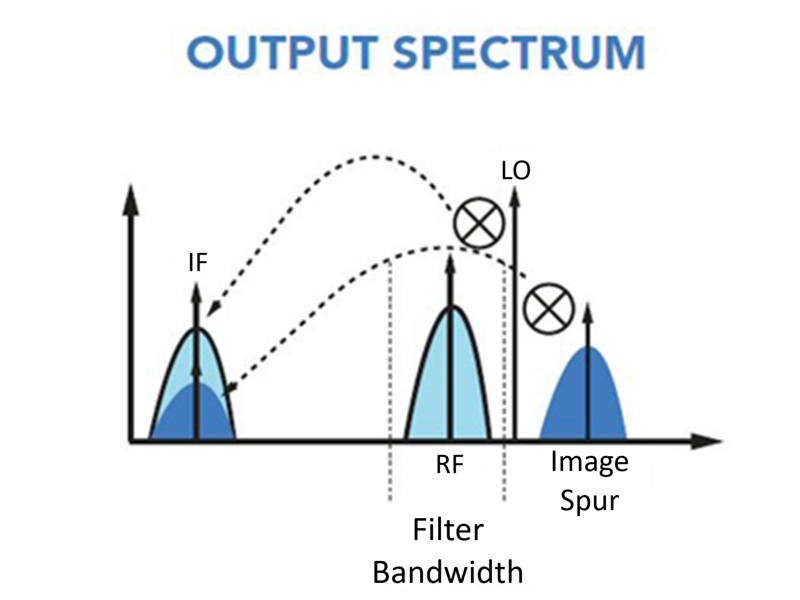
\includegraphics[scale=0.6]{MixingIllustration.jpg}
      \caption{Mixing a radio frequency (RF) signal down to an intermediate frequency (IF) (audio) signal. Shows a spur being mixed down to the same IF as the desired signal as it is the same distance from the local oscillator (LO) frequency as RF. \cite{mixing}}
    \end{figure}
    
  \end{exampleblock}


  \begin{block}{Section 1}


  \end{block}

  \begin{block}{Section 2}
  

  \end{block}


\end{column}

\separatorcolumn

\begin{column}{\colwidth}

  \begin{block}{Section 1}
    
    \begin{figure}
      \centering
      \includegraphics[scale=0.01]{sdrboard-unstuffed.jpg}
      \caption{SDR Schematic showing the analog quadrature mixer (left) and the digital controller (right).}
    \end{figure}

    \begin{figure}
      \centering
      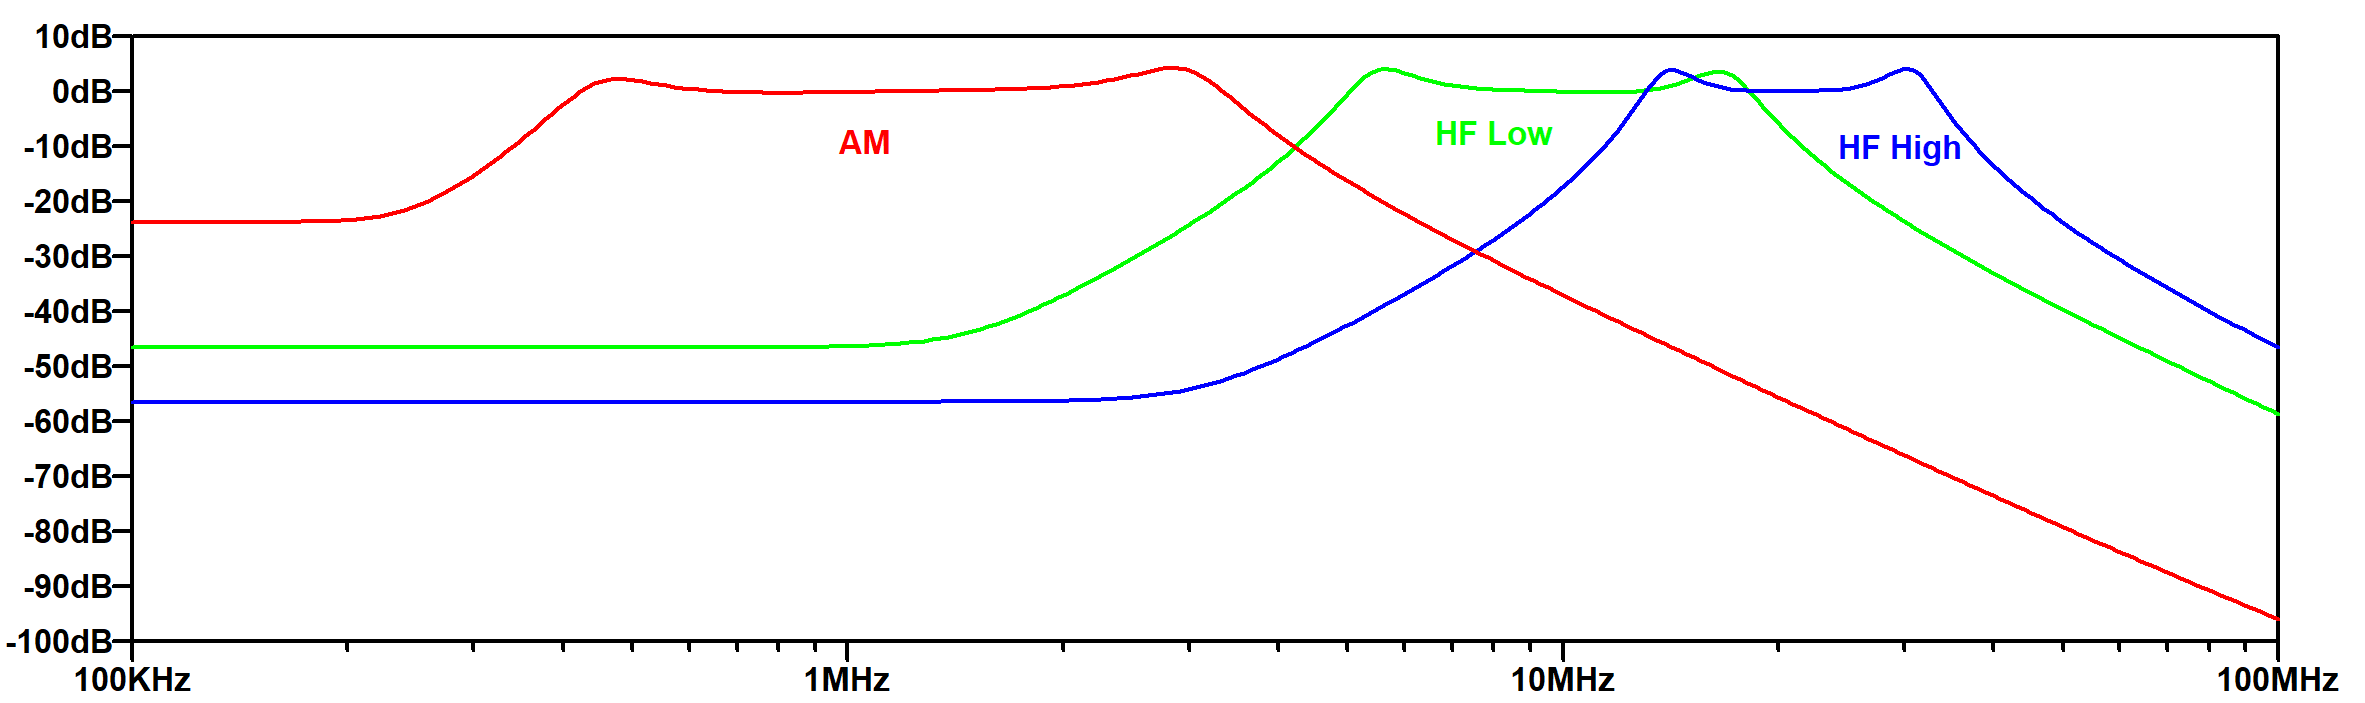
\includegraphics[scale=0.5]{bpfresponse.png}
      \caption{Simulation of the different band-pass filters.}
    \end{figure}

    \begin{figure}
      \centering
      \includegraphics[scale=0.01]{sdrboard-unstuffed.jpg}
      \caption{SDR circuit board layout. Shows the part locations and traces connecting them.}
    \end{figure}

    \begin{figure}
      \centering
      \includegraphics[scale=0.2]{sdrboard.jpg}
      \caption{The completed SDR. A physical, fully manufactured board.}
    \end{figure}

  \end{block}

  \begin{block}{Section 2}


  \end{block}


\end{column}

\separatorcolumn

\begin{column}{\colwidth}

  \begin{block}{Section 1}

    \begin{figure}
      \centering
      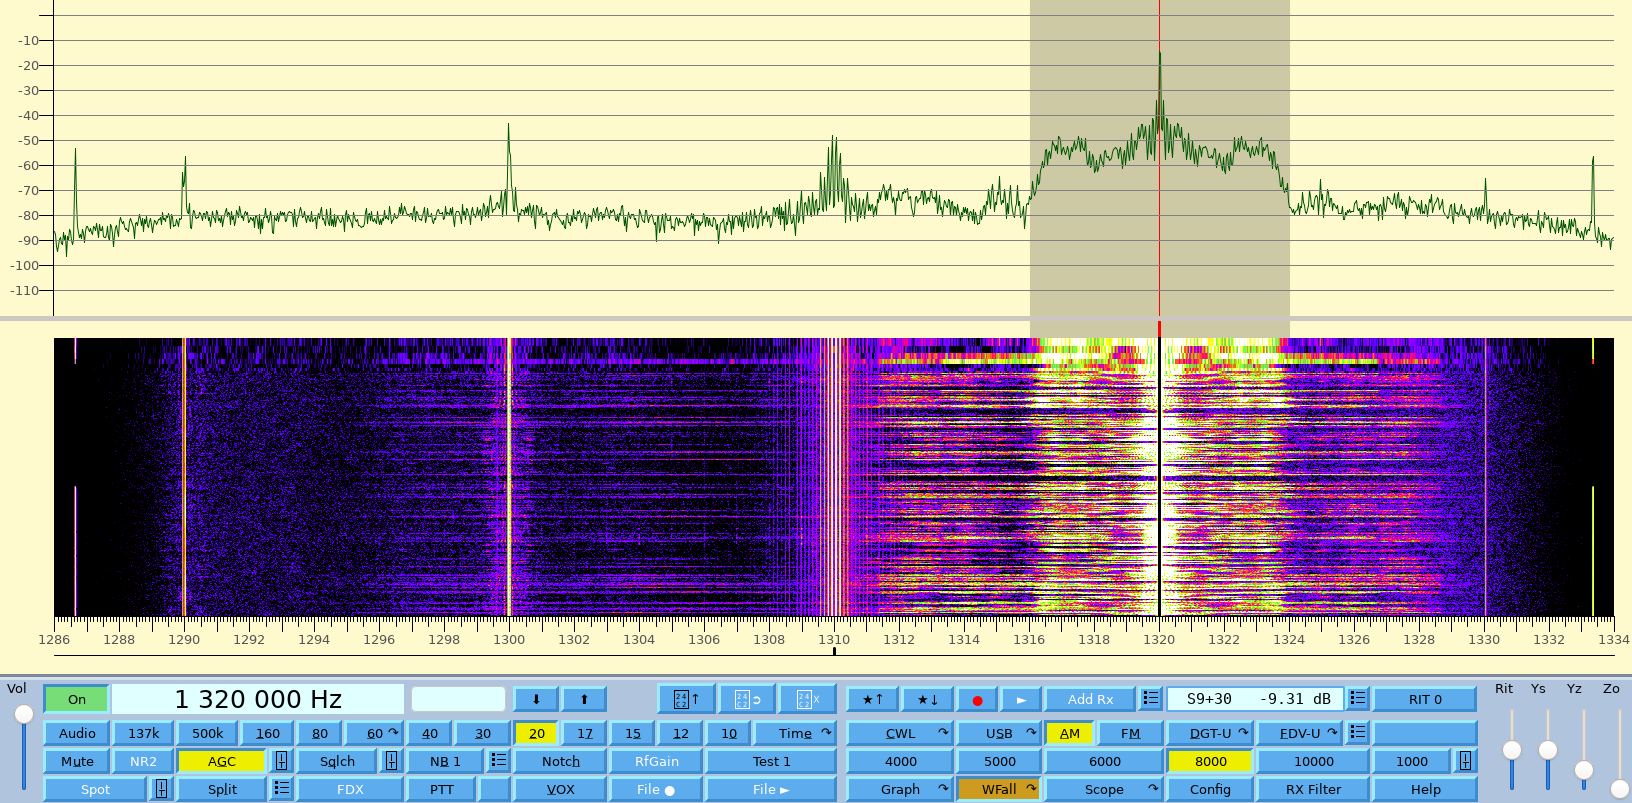
\includegraphics[scale=0.5]{quisk-am3.png}
      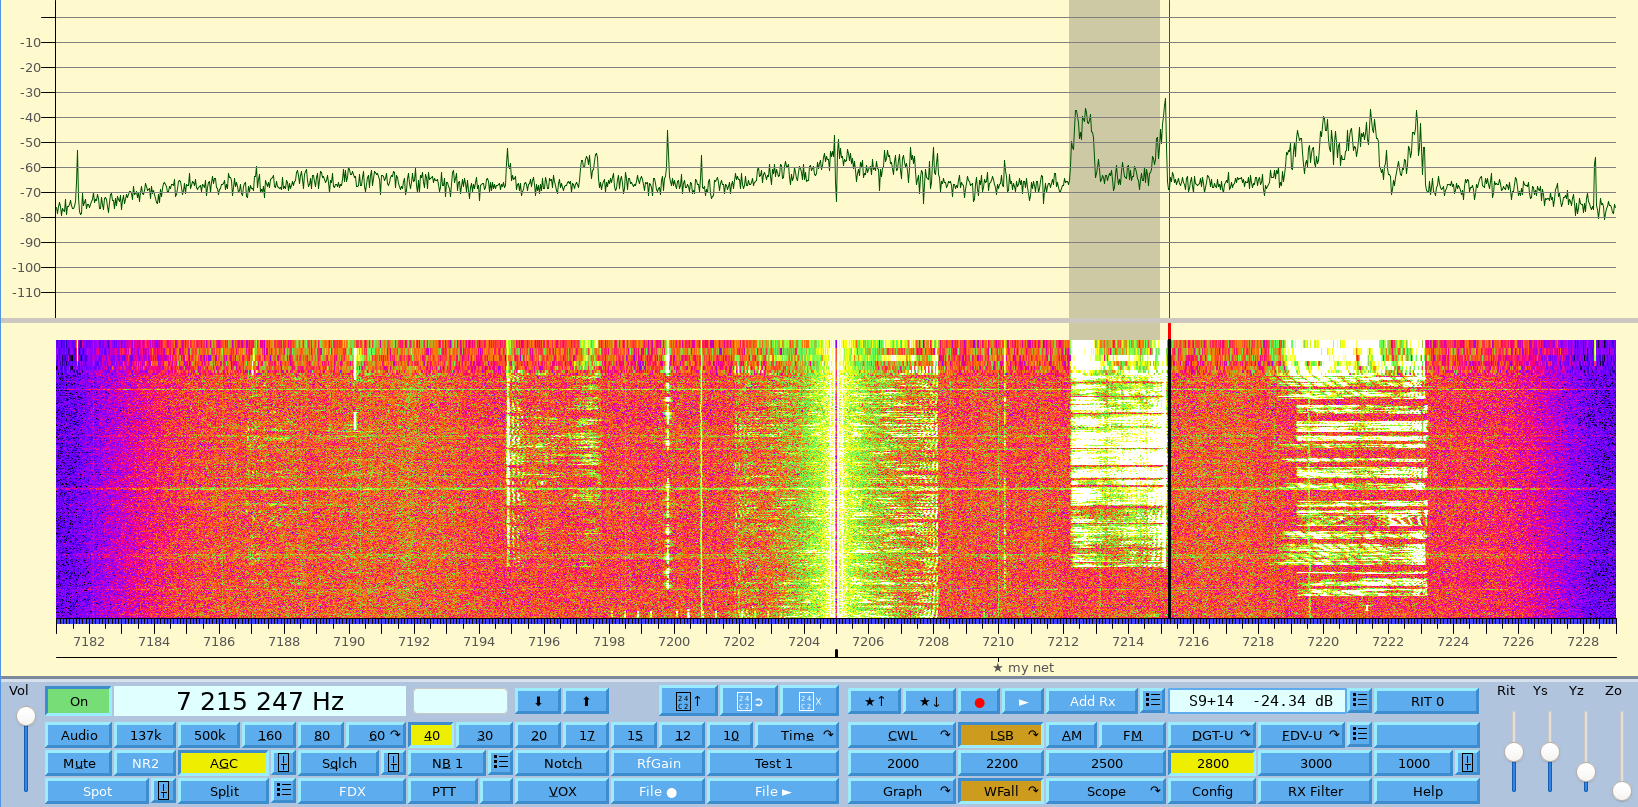
\includegraphics[scale=0.5]{quisk-ssb.png}
      \caption{Quisk SDR software \cite{quisk}. Shows the waterfall display, the audio spectrum, and device control. (Top) AM demodulation at 1.3MHz. (Bottom) SSB demodulation at 7.2MHz.}
    \end{figure}

  \end{block}
  
  \begin{block}{Section 2}

  \end{block}

  \begin{block}{References}

    \nocite{*} % don't cite everything
    \footnotesize{\bibliographystyle{plain}\bibliography{poster}}

  \end{block}

\end{column}

\separatorcolumn
\end{columns}
\end{frame}

\end{document}
